\chapter[\gls{SPECT}]{Single Photon Emission\\Computed Tomography (SPECT)}
\vspace{-45ex}
\begin{flushright}
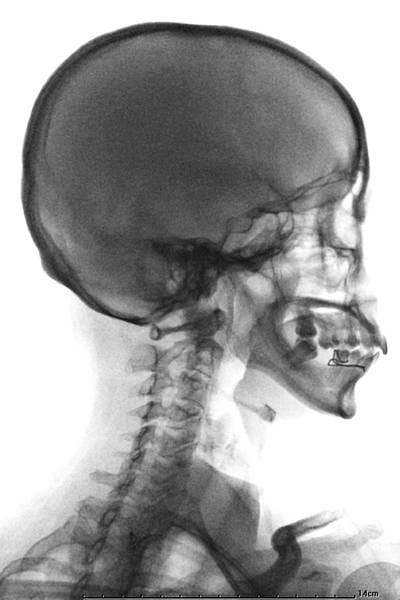
\includegraphics[width=4.5cm]{SPECT_example} % https://www.cidrad.com/wp-content/uploads/2024/06/testicular-ultrasound-riverside-county-ca-usa-near-me-400-600.jpg
\end{flushright}

\section{Acquisition}
\begin{itemize}
\item \gls{SPECT} is the tomographic counterpart of nuclear medicine
  planar imaging, just like CT is the tomographic counterpart of
  radiography \cite{bushberg2011essential}.
  
\item In SPECT, a nuclear camera records X- or Gamma-ray emissions
  from the patient from a series of different angles around the
  patient.
  
\item  These projection data are used to reconstruct a series of
  tomographic emission images.

\item The spatial resolution of the images is inversely proportional
  to the distance between the patient and of the \popup{camera}{The
    camera uses a collimator to determine the direction of the
    photons. This generates a low detection efficiency because the
    collimator filters out over 99.9\% of the emitted photons. The
    design of the collimator inherently compromises between spatial
    resolution and detection efficiency}.
\end{itemize}

\section{Clinical applications}
\begin{itemize}
\item SPECT images provide diagnostic functional information similar
  to nuclear planar examinations (functional information about organ
  physiology) ; however, their tomographic nature allows physicians to
  better understand the precise distribution of the radioactive agent,
  and to make a better assessment of the function of specific organs
  or tissues within the body.
\item The same radioactive isotopes are used in both planar nuclear
  imaging and SPECT \cite{bushberg2011essential}.
\end{itemize}

\section{Image quality}
\begin{itemize}
\item The resolution is limited (hundres of pixels in each dimension)
  by two reasons:
  \begin{enumerate}
  \item The detection efficiency (which is very low) depends on the
    pixel-size.
  \item Each projection requires dozens of seconds
    \cite{abdulla2025SPECT}.
  \end{enumerate}
\item Althought it is based on the same imaging technology than PNI,
  it usually provided improved contrast and reduced structural noise
  by averaging counts from overlapping structures
\end{itemize}